%!TEX root = ../main.tex
\chapter{Graphen}
Wir beschränken uns auf einfache ungerichtete Graphen.
\begin{definition}{Einfacher ungerichteter Graph}
	Ein \emph{einfacher ungerichteter Graph} ist ein Paar $(V,E)$ wobei $V$ die Menge der Knoten und $E\subseteq \binom V2$ die Menge der Kanten ist.
\end{definition}

\begin{definition}{Komplementgraph}
	Für einen Graph $G=(V,E)$ ist der \emph{Komplementgraph} der Graph $G'=\left(V,\binom V2\setminus E\right)$.
\end{definition}

\begin{definition}{Isomorphie}
	Zwei Graphen $G_1=(V_1,E_1)$ und $G_2=(V_2,E_2)$ sind \emph{isomorph}, falls es eine bijektive Abbildung $\varphi:V_1\rightarrow V_2$ gibt, so dass für alle $u,v\in V_1$ gilt:
	\begin{equation*}
		\simpleset{u,v}\in E_1\Leftrightarrow \simpleset{\varphi(u),\varphi(v)}\in E_2
	\end{equation*}
\end{definition}

\begin{definition}{Bipartiter Graph}
	Wenn die Knotenmenge $V$ des Graphen $G=(V,E)$ so in zwei Teile $V_1,V_2$ aufgeteilt werden kann, dass für jede Kante $\simpleset{u,v}\in E$ genau einer der beiden Knoten in $V_1$ und der andere in $V_2$ liegt, so spricht man von einem \emph{bipartiten Graphen}.
\end{definition}

Da eine Kante nach Definition eine zweielementige Menge ist, kann man für eine Kante $e$ und einen Knoten $v$ ob $v\in e$ gilt. Wir sagen dann $u$ und $e$ sind \emph{inzident}.

Zwei Knoten sind adjazent (benachbart), wenn es eine Kante zwischen ihnen gibt, d.h. $\simpleset{u,v}\in E$ bedeutet, dass $u$ und $v$ adjazent sind.

Der Grad des Knotens $u\in V$ ist die Anzahl der Kanten die zu $u$ inzident sind.

\begin{definition}{Weg}
	Ein Weg (auch Pfad) in einem Graph $(V,E)$ ist eine Folge von Knoten $(v_0,\ldots,v_n)$ von Knoten $v_i\in V$ mit der Eigenschaft, dass für alle $1\leq i\leq n$ gilt
	\begin{equation*}
	 	\simpleset{v_{i-1},v_i}\in E
	\end{equation*}
	Die Länge des Weges ist $n$, man zählt also die Anzahl durchlaufener Kanten.

	In einem einfachen Weg sind alle Knoten verschieden. 
\end{definition}
Ein Weg heißt Eulerweg, wenn auf ihm jede Kante des Graphen genau einmal durchlaufen wird.


\begin{definition}{Kreis}
	Ein Kreis ist ein Pfad, bei dem Start- und Endknoten gleich sind.

	In einem einfachen Kreis sind alle Knoten außer der erste und letzte verschieden.
\end{definition}
Ein Eulerweg der gleichzeitig ein Kreis ist, heißt Eulerkreis.

\begin{definition}{Planarität}
	Ein Graph heißt planar, wenn er sich so in die Ebene einzechnen lässt, dass sich die Kanten nicht schneiden.
\end{definition}

Eine Facette ist eine zusammenhängende Fläche, die von Kanten berandet ist, insbesondere ist das Äußere immer eine Facette.

\section{Sätze zu Graphen}
\begin{itemize}
	\item Die Summe aller Knotengrade in einem ungerichteten Graphen ist immer gerade.
	\item In jedem endlichen Graph ist die Anzahl der Knoten mit ungeradem Grad gerade.
	\item Ein zusammenhängender endlicher Graph hat genau dann einen Eulerpfad, wenn die Anzahl der Knoten mit ungeradem Grad maximal 2 ist. Ein Eulerkreis existiert genau dann, wenn alle Knoten geraden Grad haben.
	\item \textbf{Eulerformel} In endlichen zusammenhängenden planaren Graphen mit $n\geq 1$ Knoten, $m$ Kanten und $f$ Facetten gilt
	\begin{equation*}
		n-m+f=2\text{\quad bezeihungsweise\quad}n-m+f=z+1
	\end{equation*}
	für $z$ Zusammenhangskomponenten.
	Wichtige Folgerungen hieraus sind
	\begin{itemize}
		\item Ein planarer Graph mit $n\geq 3$ Knoten hat höchstens $3n-6$ Kanten.
		\item Ein planarer bipartiter Graph mit $n\geq 4$ Knoten hat höchstens $2n-4$ Kanten
		\item In jedem planaren Graph gibt es mindestens einen Knoten mit Grad kleiner oder gleich $5$.
		\item Der $K_5$ und der $K_{3,3}$ sind nicht planar.
	\end{itemize}

	\item \textbf{Satz von Kuratowski} Ein Graph ist genau dann planar, wenn er keine Unterteilung des $K_5$ oder des $K_{3,3}$ enthält.
\end{itemize}

\section{Wichtige Graphen und deren Eigenschaften}
\begin{itemize}
	\item Der $K_4$ ist der vollständige Graph mit 4 Knoten

	\begin{center}
		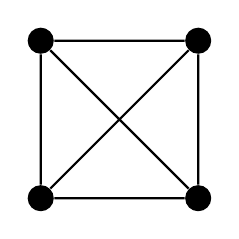
\begin{tikzpicture}
			\draw node[circle, fill=black, minimum width=4pt] (1) at (0,0) {};
			\draw node[circle, fill=black, minimum width=4pt] (2) at (2,0) {};
			\draw node[circle, fill=black, minimum width=4pt] (3) at (0,2) {};
			\draw node[circle, fill=black, minimum width=4pt] (4) at (2,2) {};

			\draw[thick] (1) -- (2) -- (3) -- (4) -- (1) -- (3) -- (4) -- (2);
		\end{tikzpicture}
	\end{center}

	Im $K_n$ haben alle Knoten den Grad $n-1$. Die Graphen $K_2=P_2,K_3=C_3$ und $K_4$ sind planar, der $K_5$ jedoch nicht.

	\item Der $P_5$ ist der Pfad-Graph mit 5 Knoten

	\begin{center}
		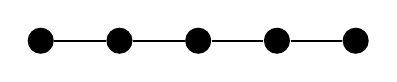
\begin{tikzpicture}
			\draw node[circle, fill=black, minimum width=4pt] (1) at (0,0) {};
			\draw node[circle, fill=black, minimum width=4pt] (2) at (1,0) {};
			\draw node[circle, fill=black, minimum width=4pt] (3) at (2,0) {};
			\draw node[circle, fill=black, minimum width=4pt] (4) at (3,0) {};
			\draw node[circle, fill=black, minimum width=4pt] (5) at (4,0) {};

			\draw[thick] (1) -- (2) -- (3) -- (4) -- (5);
		\end{tikzpicture}
	\end{center}

	Der $P_n$ hat für $n\geq 2$ immer einen Eulerweg aber keinen Eulerkreis. Alle $P_n$ sind planar.

	\item Der $C_6$ ist der Kreis-Graph mit 6 Knoten
	\begin{center}
		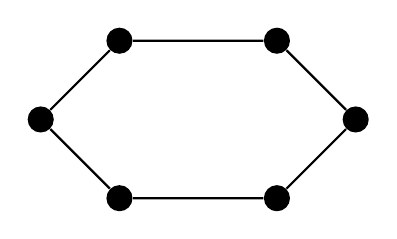
\begin{tikzpicture}
			\draw node[circle, fill=black, minimum width=4pt] (1) at (0,0) {};
			\draw node[circle, fill=black, minimum width=4pt] (2) at (2,0) {};
			\draw node[circle, fill=black, minimum width=4pt] (3) at (3,1) {};
			\draw node[circle, fill=black, minimum width=4pt] (4) at (2,2) {};
			\draw node[circle, fill=black, minimum width=4pt] (5) at (0,2) {};
			\draw node[circle, fill=black, minimum width=4pt] (6) at (-1,1) {};

			\draw[thick] (1) -- (2) -- (3) -- (4) -- (5) -- (6) -- (1);
		\end{tikzpicture}
	\end{center}

	Der kleinste Kreis-Graph ist der $C_3$.

	Der $C_n$ hat immer einen Eulerkreis. 

	Alle $C_n$ sind planar.

	Im $C_n$ hat jeder Knoten hat den Grad 2. 

	\item Der $K_{3,3}$ ist der bipartite Graph mit jeweils 3 Knoten in einer Partition

	\begin{center}
		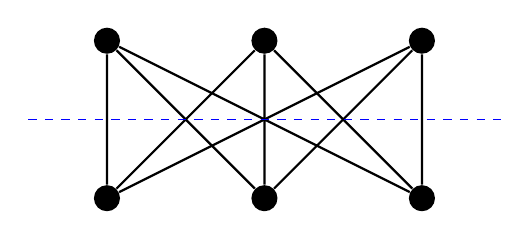
\begin{tikzpicture}
			\draw node[circle, fill=black, minimum width=4pt] (1) at (0,2) {};
			\draw node[circle, fill=black, minimum width=4pt] (2) at (2,2) {};
			\draw node[circle, fill=black, minimum width=4pt] (3) at (4,2) {};
			\draw node[circle, fill=black, minimum width=4pt] (4) at (0,0) {};
			\draw node[circle, fill=black, minimum width=4pt] (5) at (2,0) {};
			\draw node[circle, fill=black, minimum width=4pt] (6) at (4,0) {};

			\draw[thick] (1) -- (4) -- (2) -- (5) -- (1) -- (6) -- (3) -- (5);
			\draw[thick] (4) -- (3);
			\draw[thick] (2) -- (6);

			\draw[blue, dashed] (-1,1) -- (5,1);
		\end{tikzpicture}
	\end{center}

	Im $K_{3,3}$ hat jeder Knoten den Grad $3$.

	Der $K_{3,3}$ ist nicht planar.
\end{itemize}